\begin{center}
\fbox{\fbox{\parbox{6.5in}{\centering
\begin{flushleft}

\vspace{2mm}
\hspace{5mm}
\textbf{\underline{Trapets}}

\vspace{2mm}
\hspace{5mm}
Trapets on nelinurk, mille \textbf{kaks külge on paralleelsed} ja kaks mitteparalleelsed.

\vspace{2mm}
\hspace{5mm}
Paralleelseid külgi nimetatakse \textbf{alusteks} ning nende vahelist kaugust trapetsi \textbf{kõrguseks}.\\ \hspace{5mm} Mitte paralleelseid külgi nimetatakse \textbf{haaradeks}.

\vspace{5mm}
\hspace{5mm}
\begin{tikzpicture}[scale=0.4, bullet/.style={circle,fill,inner sep=1pt}]

\coordinate (A) at (-4,-2);
\coordinate (B) at (0,2);
\coordinate (C) at (6,2);
\coordinate (D) at (7,-2);
\coordinate (h) at (0,-2);

\draw (A)--(B)--(C)--(D)--cycle; 
\node[left] at (A){$A$};
\node[left] at (B){$B$};
\node[right] at (C){$C$};
\node[right] at (D){$D$};



\path (A)--(B) coordinate[pos=0.5](a);
\path (B)--(C) coordinate[pos=0.5](b);
\path (C)--(D) coordinate[pos=0.5](c);
\path (D)--(A) coordinate[pos=0.5](e);
\node[left] at (a){$c$};
\node[above] at (b){$b$};
\node[right] at (c){$e$};
\node[below] at (e){$a$};

\path (B)--(h) coordinate[pos=0.5](h1);
\node[right] at (h1){$h$};
\draw[dashed] (B)--(h);
\pic [draw,angle radius=4mm] {angle=D--h--B};
\node[bullet, above right] at (0.3,-1.7){};

\node[text width=4cm]at(18,0){$a$ ja $b$ on alused.\\
$h$ on kõrgus.\\
$c$ ja $e$ on haarad.};
\end{tikzpicture}

\vspace{5mm}
\hspace{5mm}
\textbf{\underline{Võrdhaarne trapets}}

\vspace{2mm}
\hspace{5mm}
Kui trapetsi haarad on võrdsed (ehk võrdse pikkusega), siis nimetatakse seda trapetsit \textbf{võrdhaarseks}.

\vspace{2mm}
\hspace{5mm}
\begin{tikzpicture}[scale=0.4]

\coordinate (A) at (-2,-2);
\coordinate (B) at (0,2);
\coordinate (C) at (5,2);
\coordinate (D) at (7, -2);

\draw (A)--(B)--(C)--(D)--cycle;

\node[below] at (A){$A$};
\node[above] at (B){$B$};
\node[above] at (C){$C$};
\node[below] at (D){$D$};
\pic [draw,angle radius=4mm] {angle=D--A--B};
\pic [draw,angle radius=4mm] {angle=C--D--A};
\pic [draw,angle radius=4mm] {angle=A--B--C};
\pic [draw,angle radius=4mm] {angle=B--C--D};
\pic [draw,angle radius=3.5mm] {angle=A--B--C};
\pic [draw,angle radius=3.5mm] {angle=B--C--D};

\tkzMarkSegment[color=black,pos=.5,mark=|](A,B) 
\tkzMarkSegment[color=black,pos=.5,mark=|](C,D) 

\path (A)--(D) coordinate[pos=0.5](a);
\node[below] at (a){$a$};
\path (A)--(B) coordinate[pos=0.5](c1);
\node[above left] at (c1){$c$};
\path(B)--(C) coordinate[pos=0.5](b);
\node[above] at (b){$b$};
\path (C)--(D) coordinate[pos=0.5](c2);
\node[above right] at (c2){$c$};

\node[text width=8cm] at (20,0) {Võrdhaarne trapets on sümmeetriline.\\
Võrdhaarse trapetsi mõlema aluse lähisnurgad on võrdsed.};

\end{tikzpicture}

\vspace{5mm}
\hspace{5mm}
\textbf{\underline{Täisnurkne trapets}}

\vspace{2mm}
\hspace{5mm}
Kui üks trapetsi haaradest on risti ($\perp$) kummagi alusega, siis on tegemist \textbf{täisnurkse trapetsiga}.

\vspace{5mm}
\hspace{5mm}
\begin{tikzpicture}[scale=0.4]

\coordinate (A) at (0,-2);
\coordinate (B) at (0,2);
\coordinate (C) at (5,2);
\coordinate (D) at (9,-2);

\draw (A)--(B)--(C)--(D)--cycle;

\node[left] at (A) {$A$};
\node[above] at (B){$B$};
\node[above] at (C){$C$};
\node[right] at (D){$D$};

\path (A)--(B) coordinate[pos=0.5](a);
\node[left] at (a) {$h$};
\path (B)--(C) coordinate[pos=0.5](b);
\node[above] at (b) {$b$};
\path (C)--(D) coordinate[pos=0.5](c);
\node[right] at (c) {$c$};
\path (D)--(A) coordinate[pos=0.5](h);
\node[below] at (h) {$a$};


\pic [draw,angle radius=4mm] {angle=A--B--C};
\pic [draw,angle radius=4mm] {angle=D--A--B};

\node[above right] at (0.25, -1.75)[circle,fill,inner sep=1pt]{};
\node[below right] at (0.25, 1.75)[circle,fill,inner sep=1pt]{};

\node[text width=8cm] at (22,0) {Täisnurkse trapetsi puhul on lühem haar (ehk haar, mis on alustega risti) võrdne ka trapetsi kõrgusega.};
\end{tikzpicture} 

\vspace{5mm}
\hspace{5mm}
\textbf{\underline{Trapetsi pindala valem}}

\vspace{2mm}
\hspace{5mm}
Trapetsi pindala: $\boxed{S=\dfrac{a+b}{2}\cdot h}$

\vspace{4mm}
\hspace{5mm}
kus $a$ ja $b$ on trapetsi alused ning $h$ on trapetsi kõrgus.

\end{flushleft}
}}}
\end{center}





\begin{center}
\fbox{\fbox{\parbox{6.5in}{\centering
\begin{flushleft}


\vspace{2mm}
\hspace{5mm}
\textbf{\underline{Kolmnurga kesklõik}}

\vspace{2mm}
\hspace{5mm}
\textbf{Kolmnurga kesklõik} - lõik, mis ühendab kolmnurga kahe külje keskpunkte.


\vspace{2mm}
\hspace{5mm}
\begin{tikzpicture}[scale=0.5]
\coordinate (A) at (0,0);
\coordinate (B) at (2,4);
\coordinate (C) at (7,0);

\node[below] at (A){$A$};
\node[above] at (B){$B$};
\node[below] at (C){$C$};


\draw (A)--(B)--(C)--cycle;
\path (A)--(B) coordinate[pos=0.5](k1);
\path (B)--(C) coordinate[pos=0.5](k2);
\draw[dashed] (k1)--(k2);
\path (k1)--(k2) coordinate[pos=0.5](kesklõik);
\node[below] at (kesklõik){$k$};


\node[left] at (k1){$D$};
\node[right] at (k2){$E$};

\tkzMarkSegment[color=black,pos=.5,mark=|](A,k1);
\tkzMarkSegment[color=black,pos=.5,mark=|](k1,B);

\tkzMarkSegment[color=black,pos=.5,mark=||](B,k2);
\tkzMarkSegment[color=black,pos=.5,mark=||](k2,C);   

\path (A)--(C) coordinate[pos=0.5](alus);
\node[below] at (alus){$a$};

\node [text width=9cm] at (18,2){Igal kolmnurgal on kolm kesklõiku.\\
\vspace{2mm}
Kolmnurga kesklõik on paralleelne kolmnurga ühe küljega ja on pool sellest küljest (millega ta paralleelne on).\\
Ehk: $AC \parallel DE$ ja $DE=\dfrac{1}{2}AC$.};
\end{tikzpicture}

\vspace{5mm}
\hspace{5mm}
\textbf{\underline{Trapetsi kesklõik}}

\vspace{2mm}
\hspace{5mm}
\textbf{Trapetsi kesklõik} - lõik, mis ühendab trapetsi haarade keskpunkte.

\vspace{5mm}
\hspace{5mm}
\begin{tikzpicture}[scale=0.4]
\coordinate (A) at (0,-2);
\coordinate (B) at (3,2);
\coordinate (C) at (7,2);
\coordinate (D) at (8,-2);

\draw (A)--(B)--(C)--(D)--cycle;
\node[below] at (A){$A$};
\node[above] at (B){$B$};
\node[above] at (C){$C$};
\node[below] at (D){$D$};

\path (A)--(B) coordinate[pos=0.5](k1);
\path (C)--(D) coordinate[pos=0.5](k2);
\draw[dashed] (k1)--(k2);
\path (k1)--(k2) coordinate[pos=0.5](kesklõik);
\node[below] at (kesklõik){$k$};

\node[left] at (k1){$D$};
\node[right] at (k2){$E$};

\tkzMarkSegment[color=black,pos=.5,mark=|](A,k1);
\tkzMarkSegment[color=black,pos=.5,mark=|](k1,B);

\tkzMarkSegment[color=black,pos=.5,mark=||](C,k2);
\tkzMarkSegment[color=black,pos=.5,mark=||](k2,D);   

\path (A)--(D) coordinate[pos=0.5](alus);
\node[below] at (alus){$a$};

\node [text width=9cm] at (22.5,0){Igal trapetsil on vaid üks kesklõik.\\
\vspace{2mm}
Trapetsi kesklõik on paralleelne trapetsi mõlema alusega ja võrdub aluste poolsummaga (ehk nende aritmeetilise keskmisega).\\
Ehk: $AD \parallel DE \parallel BC$ ja $DE=\dfrac{AD+BC}{2}$.};

\end{tikzpicture}

\vspace{5mm}
\hspace{5mm}
\textbf{\underline{Kesklõigu kaudu avaldatud pindala valemid}}

\vspace{2mm}
\hspace{5mm}
Nii kolmnurga kui ka trapetsi pindalad võrduvad kesklõigu $k$ ja kõrguse $h$ korrutisega.

\vspace{2mm}
\hspace{5mm}
Ehk: $\boxed{S_{k}=kh}$ ja $\boxed{S_{t}=kh}$

\vspace{2mm}
\hspace{5mm}
kus $S_{k}$ - kolmnurga pindala, $S_{t}$ - trapetsi pindala, $k$ - kesklõik, $ h$ - kolmnurga või trapetsi kõrgus.

\end{flushleft}
}}}
\end{center}

\vspace{0.5cm}

\textbf{Märkmed}\\
\vspace{2mm}
\begin{mdframed}[style=graphpaper]
\vspace{7cm}
\end{mdframed}